\documentclass[twoside,11pt]{article}

% Any additional packages needed should be included after jmlr2e.
% Note that jmlr2e.sty includes epsfig, amssymb, natbib and graphicx,
% and defines many common macros, such as 'proof' and 'example'.
%
% It also sets the bibliographystyle to plainnat; for more information on
% natbib citation styles, see the natbib documentation, a copy of which
% is archived at http://www.jmlr.org/format/natbib.pdf

\usepackage{jmlr2e}
\usepackage{braket}
\usepackage[]{algorithm2e}
\usepackage{multirow}
\usepackage{mathrsfs}
\usepackage[Symbol]{upgreek}
\usepackage{mathtools}
\usepackage{fancyref}
\usepackage{graphicx}
%\usepackage{placeins}
\usepackage{subcaption}
\usepackage{fixltx2e}
% Definitions of handy macros can go here

\newcommand{\dataset}{{\cal D}}
\newcommand{\fracpartial}[2]{\frac{\partial #1}{\partial  #2}}

% Heading arguments are {volume}{year}{pages}{submitted}{published}{author-full-names}

\jmlrheading{1}{2000}{1-48}{4/00}{10/00}{Name and Name}

% Short headings should be running head and authors last names

\ShortHeadings{Imitation Learning for Accelerating Fixed Point Iterative Processes }{Name and Name}
\firstpageno{1}

\begin{document}

\title{Imitation Learning for Accelerating Iterative Computation of Fixed Points}
%title{Speeding up Hartree-Fock by Imitation Learning}
% MT, Tse-Han, Geoff, Dave

\author{\name Name\ Name \email email \\
       \addr Department\\
       University \\
       City, State , USA
       \AND
       \name Name\ Name \email email \\
       \addr Department\\
       University \\
       City, State , USA}
\editor{editor name}

\maketitle

% todo:
% talk about differentiating through HF to get gradients?
% do we ever use parameterized HF in this work?  (e.g., scale some of the integrals)

\begin{abstract}%
Many computational methods in science and engineering work by fixed-point iteration---repeatedly applying a given update function until convergence.  Unfortunately, this sort of iterative computation can be expensive: the update function itself may be costly to compute, and we may need many updates before we reach the desired fixed point.  So, we explore a means to accelerate fixed-point iteration via imitation learning.  Our approach is simple and appealing, and needs only black-box access to the original update function.  We show in experiments that our approach successfully accelerates a central algorithm from quantum chemistry: the Hartree-Fock method for calculating the electronic structure and energy of a molecular system.  Our results indicate that policies trained on one set of molecules transfer successfully to other molecules of the same general class.  They also indicate that imitation learning leads to more-robust transfer compared to alternative methods that do not take into account the distribution of states induced by our learned policies.
%
% We use this access to construct expert demonstrations that take larger steps through the sequence of iterates. In the current studies, the convergence rate is doubled by eliminating odd-numbered iterates. A policy that mimics this enhanced expert performance is then trained using the Dataset Aggregation algorithm (DAgger), which learns a policy that is guaranteed to perform well under its induced distribution of states. The studies are carried out using the Hartree-Fock fixed-point algorithm of quantum chemistry, which is a mean-field theory of the electronic structure and energy of a molecular system. The results indicate that policies trained on a set of molecules transfer successfully to other molecules of the same general class. The DAgger algorithm leads to more robust transfer than alternative methods that do include training on the distribution of states induced by the learned policies.
\end{abstract}

\section{INTRODUCTION}

% GJG: at some point we should probably compare: just swap in a deep net instead of using HF update calculation at all

Many computational methods in science and engineering use fixed-point iteration
\[
x_{n+1} = f(x_n), \quad n = 0,1,2,3...
\]
to attempt to find fixed points of $f$, i.e., points at which $f(x)=x$. These methods generate a sequence of iterates, $x_0, x_1, x_2, \ldots$, that ideally converge to a fixed point $x$. This paper explores the application of imitation learning to fixed-point iteration to accelerate convergence and improve stability. Imitation learning, also called learning from demonstration, is designed to learn a policy that imitates an expert's method of performing a target task: we gather training data by posing task instances to the expert, and train a function approximator to mimic the expert's mapping from situations to actions.

The most straightforward way to apply imitation learning to fixed-point calculations would be to treat our original update function as the expert: we would train a cheaper function approximator to imitate the original, more expensive expert update function, and hopefully gain the ability to perform each iteration of our algorithm faster without losing significant accuracy in the final fixed point.  
%
However, scientific and engineering applications often have two important differences from typical uses of imitation learning, making the straightforward approach problematic.  First, to achieve a useful speedup, we do not need to completely eliminate calls to the expert update function; it is enough to reduce their frequency.  Second, considerable effort has often gone into developing and fine-tuning the expert; simply replacing the expert update function with a naive function approximator would throw away much of this effort.  In particular, the expert update function often encodes physical constraints and intuitions that would be difficult to enforce with a naive function approximator; dropping these constraints and intuitions would lead to solutions that are not acceptable to domain experts, even if we were able to maintain or improve overall approximation error.

So instead of completely replacing the expert, we propose to train our imitation learner to skip some of the steps from our original sequence of iterates: given the \emph{output} of the expert at step $t$, the learner tries to predict a good \emph{input} for the expert at step $t+\Delta$.  By doing so, we replace two or more calls to the expensive expert with a single call, saving computation; but we still only task our learner with the easier job of producing a good input to the expert instead of mimicking its output.  The difference is that, unlike the output, the input need not respect physical constraints or intuitions: we assume that the expert itself is responsible for enforcing these, and is capable of repairing small violations.

% For many important problems in science and engineering, considerable effort has gone into developing and fine-tuning fixed-point iteration algorithms. The sequences generated from these existing algorithms, $x_0, x_1, x_2, \ldots$  provide a basis for creating expert demonstrations with enhanced performance. For example, the series $x_0, x_2, x_4, \ldots$ provides an enhanced expert demonstration with accelerated convergence. The use of imitation learning to discover policies that mimic the behavior of such enhanced experts has the potential to substantially improve algorithms that are at the core of much of computational science.

As a test case for our methodology, we accelerate the Hartree-Fock method from computational quantum chemistry. Hartree-Fock is a fixed-point algorithm that approximates the electronic structure and energy of molecules.  It is a specific instance of a broader class of mean-field-theory approaches to many-body problems. In such mean-field theories, the effect of all individuals on any given individual is approximated by a single averaged effect, thus reducing a many-body problem to a one-body problem. In quantum chemistry, the mean field arises from the averaged charge distribution of all electrons, as described by the electron density, $\rho({\bf r})$. The Hartree-Fock iterations thereby generate a sequence of electron densities that ideally converge to a fixed point. Quantum chemical methods that go beyond mean-field theory typically begin with the results of a Hartree-Fock calculation, making the Hartree-Fock algorithm a pervasive component of quantum chemistry~\cite{Some authoritative review of electronic structure theory}.

% Here, well-established Hartree-Fock algorithms are used to generate series of electron densities from which enhanced expert demonstrations are constructed. We then apply supervised learning to train a policy that mimics the demonstration. However, naive supervised learning may yield poor performance in practice and also in theory.  Because the learner's prediction and action affect future observations and states during the execution of the learned policy, it obviously violates the common i.i.d. assumption made in most statistical learning approaches \citep{Ross}. Fortunately, the dataset aggregation algorithm (DAgger), proposed by Ross et al. \citep{DAgger}, can learn a stationary deterministic policy guaranteed to perform well under its induced distribution of states. This in turn serves as a remedy to the poor performance in naive supervised learning. DAgger also has been shown to have stable performance and fast learning rate \citep{DAggerCompare}. Below, DAgger is shown to yield policies whose performance is superior to those obtained from more naive approaches. 

\section{BACKGROUND}

\subsection{Hartree-Fock}
% GJG: I moved a lot of stuff to an appendix
% also note: I suppressed the phrase "atomic orbital"
% also note: added detail to HF iteration and mostly rewrote this section PLEASE CHECK
% also note: changed iteration counter to t (i gets used for tons of other stuff...)
% changed C^TC to CC^T
The core problem of quantum chemistry is to compute the distribution of electrons in a molecule given the positions of its nuclei.  The Hartree-Fock method efficiently approximates this electron distribution.  From a computational standpoint, the relevant properties of Hartree-Fock are:
\begin{itemize}
\item It is a fixed-point algorithm, whose iterates are single-electron density functions $\rho(\mathbf r)$, represented as symmetric matrices using a fixed set of basis functions $\{\chi_i(\mathbf r)\}_{i=1}^{N_{\rm basis}}$.
\item The basis set size $N_{\rm basis}$ is typically at least linear in the number of nuclei in the molecule we are considering.
\item Each iteration of Hartree-Fock is expensive: among other operations, we must iterate over all 4-tuples of basis functions to construct our mean-field approximation (nominally taking $O(N_{\rm basis}^4)$ time, although scalings closer to $O(N_{\rm basis}^3)$ are routinely achieved by taking advantage of sparsity~\ref{?}).
% GJG: we also need to find the bottom N/2 eigenvalues/vectors of an N_basis^2 matrix -- I assume that this is cheaper than constructing G?
\end{itemize}
The Hartree-Fock method is shown as Algorithm~\ref{alg:hf}, and a more detailed explanation is provided in Appendix~\ref{app:hf}.  The lines inside the \textbf{while} loop constitute the fixed point update step, mapping $\rho_i$ to $\rho_{i+1}$.

\begin{algorithm}[htb]
 \KwData{ Coordinates of atomic nuclei; basis set $\chi_i$; number of electrons $N$; initial density matrix $\rho_0$; termination criterion $\delta>0$}
 \KwResult{Density matrix with approximately-minimum energy}
	Calculate overlap matrix: $S_{ij}\leftarrow \langle \chi_i, \chi_j\rangle$ \\
	Initialize $t \leftarrow 0$ \\	
 \While{ $t=0$ or $|E_{t} - E_{t-1}| > \delta$ }{
	Calculate the Fock matrix $F\leftarrow F(\rho_t)$\\
	Solve generalized eigenproblem $Fc = \epsilon Sc$ for eigenpairs $c_a,\epsilon_a$\\
	Build matrix $C$: stack eigenvectors $c_a$ side by side, two copies of each, starting from lowest energy $\epsilon_a$, until we have added $N$ columns\\
	Update density matrix $\rho_{t+1}$ = $CC^\top$\\
    Update energy $E_{t+1}\leftarrow$ sum of $\epsilon_a$ for columns of $C$\\
	$t \leftarrow t+1$ \\
 }
 \caption{Hartree-Fock}
\label{alg:hf}
\end{algorithm}

% \begin{algorithm}[htb]
%  \KwData{ 3D coordinates of atomic nuclei}
%  \KwResult{Density matrix which gives minimum energy}
% 	Choose basis set of desired size \\
% 	Initialize $i \leftarrow 0$ \\	
% 	Pick a starting density matrix $\rho_0$ \\
% 	Pick $\delta>0$ (termination criterion) \\
%  \While{ $i=0$ or $|E_{i} - E_{i-1}| > \delta$ }{
%     % Construct guess density matrix $\rho$ from available $\rho_i$ \\
% 	Calculate the Fock operator $F \leftarrow h_1 + G(\rho_i)$\\
% 	Solve for $\epsilon$ and $C$ using Eq.~\ref{eq:fockMatrix} \\
% 	Update density matrix $\rho_{i+1}$ = $C^TC$\\
% 	$i \leftarrow i+1$ \\
%  }
%  \caption{Hartree-Fock}
% \label{alg:hf}
% \end{algorithm}

A number of extensions to the base Hartree-Fock method have been proposed; most relevant to the current study is an approach called Direct Inversion in the Iterative Subspace, or DIIS \citep{Pulay1980}.  In DIIS, we no longer take the output of iteration $t$ directly as the input to iteration $t+1$.  Instead, at the beginning of iteration $t$, we build an input density matrix $\rho'_{t}$ as a linear combination of the past several output density matrices $\rho_t, \rho_{t-1}, \rho_{t-2}, \ldots$, and use $\rho'_{t}$ to calculate the Fock operator $\hat F$ in the first line of the \textbf{while} loop.  The coefficients of the linear combination are chosen by minimizing some measure of the error of the resulting iterates.  Various methods have been used to define the error measure and to find the weights that minimize it~\citep{ADIIS,compScuseria,Alejandro2012}. However, identifying weights that lead to the fastest and most stable convergence remains an open question~\citep{Konstantin2002, Thorsten2011}.

The relevance of DIIS is that its overall form is the same as that of our proposed method: we train a function approximator (in this case linear regression) to produce a good input to an expert-designed fixed-point update step (in this case the Hartree-Fock update).  In contrast to existing DIIS methods, however, we view the problem of training our function approximator as one of imitation learning: we explicitly take into account the effect of our learned weights, not just on the immediate error, but on the overall degree to which the fixed-point iteration tracks the behavior of our expert policy.  By so doing, we hope to achieve faster and more stable convergence than existing methods.

%GEOFF: Moved this section to right before the full description of the method. Is that ok?
%\subsection{Accelerating Hartree-Fock convergence as an imitation learning problem}

%The $n$ iterations of the Hartree-Fock process may be viewed as a sequence, beginning with the initial density matrix $\rho_0$, moving through $n-1$ intermediate density matrices $\rho_1$,  $\rho_2$,  $\ldots$ ,$\rho_{n-1}$ and finally ending at the steady-state converged output $\rho_{n}$. The only object that is needed is the final steady-state density matrix. If we can get this final density matrices with fewer iterations, the computation time would be shortened. An expert demonstration with twice the original convergence rate can be constructed, for example, by taking a step size of 2 over the original trajectory: $\rho_0 \rightarrow \rho_2 \rightarrow  \rho_4 \rightarrow  \ldots \rightarrow  \rho_{n}$. We can also construction greedier trajectories by taking larger step sizes or by moving directly to the steady-state density matrix from any starting point ($\rho_0 \rightarrow \rho_{n}$). 

%The connection to imitation learning is through the attempt to learn policies that map from any input density matrix to the next density matrix of one of these accelerated sequences. Below, these policies are invoked in the first line of the while loop in Algorithm~\ref{alg:hf}, where the density matrix to be used to compute the Fock matrix is constructed from the density matrices obtained from past iterations. 

\subsection{Imitation learning}

In imitation learning, we wish to discover how to solve a sequential decision problem by using expert demonstrations.  We are given access to the expert's policy $\pi^*$, which is a (possibly randomized) mapping from states of the world $s$ to actions $a=\pi^*(s)$.  And, we are given access to a world model $M$: for any state $s$ and action $a$, $M$ is a (possibly randomized) mapping to the next state $s'=M(s,a)$.
Using the policy and the world model we can sample training trajectories: for each trajectory, we start in some state $s_1$, execute action $a_1=\pi^*(s_1)$, transition to state $s_2=M(s_1,a_1)$, and repeat for some number of steps.  We can then use these trajectories to train a predictor that, given the current state, predicts the expert's action.
The key difficulty in imitation learning is that prediction errors early in a trajectory can cause us to deviate from the expert's distribution over states; so, we can easily drift into areas of the state space where we have little or no training data, causing a growing cascade of errors.

%GEOFF: We substantially re-wrote this section. Please check to make sure we got it correct.
In our experiments, we use the DAgger algorithm for imitation learning \citep{DAgger}.  DAgger (Algorithm~\ref{alg:DAgger}) avoids the above difficulty by using its current hypothesized policy at each iteration to gather additional training trajectories, so that it gains experience on how to correct its own errors.
%
%In each iteration, DAgger trains a model under the states that were induced by both the expert and the previous learned models. This aggregation expands the training to include inputs that the model is likely to encounter based on previous training iterations. By doing so, it is possible to offset the error made by previous learned models and thus learn a new policy that better approaches the demonstration. This is a remedy to the problem, in naive supervised learning, that the error may grow quadratically and results may become unpredictable because the policy is trained under a different state distribution than the model may encounter. 
%
In Algorithm~\ref{alg:DAgger}, $\Pi$ is the class of policies the learner is considering: in our case, taking a linear combination of past density matrices as input to a step of Hartree-Fock. In the first iteration, DAgger uses the expert's policy $\pi^*$ to gather a dataset of trajectories $D$ and train a policy $\hat{\pi}_2$ that best mimics the expert on those trajectories. 
Then in iteration $j$, DAgger samples states according to a mixture of policies ($\hat{\pi}_j$ and the expert $\pi^*$, mixed with probability $\beta_j$) and refers to the expert's action on these states, forming the dataset $D_j$, which is in turn added to the overall dataset $D$. We then train the next policy $\hat{\pi}_{j+1}$, the policy that best mimics the expert on the combined dataset $D$.  

%The process is then repeated to further rectify the error produced by the policy learned in the previous iteration until we reach iteration $N$.

\begin{algorithm}[htb]
 \KwData{Expert's demonstration generated by expert's policy $\pi^*$}
 \KwResult{Best $\hat{\pi}_j$ on validation }
 $\pi^*$  is the expert’s policy \\
 Initialized $D \leftarrow \emptyset$ \\
 Initialized $\hat{\pi}_1$ to any policy in $\Pi$ \\
 \For{j=1 to N }{
    %GEOFF: Assume beta is a sampling probability. Does this need to be defined the main text?
    % GJG: probably should define beta in main text
	Let $\pi_j$ = $\beta_{j}\pi^* + (1-\beta_{j})\hat{\pi}_j$ \\
	Sample T-step trajectories using $\pi_j$ \\
	Get dataset $D_j$ = \{(s, $\pi^*$(s))\} of visited states by $\pi_j$ and actions given by expert. \\
	Aggregate datasets: $D \leftarrow D \cup D_j$ \\
	Train policy $\hat{\pi}_{j+1}$ on $D$\\
 }
 \caption{DAgger}
 \label{alg:DAgger}
\end{algorithm}

\section{LEARNING THE POLICY} \label{sec:policy}

% GJG: state policy form explicitly: linear combo followed by HF step
% GJG: state form of expert explicitly: it is to map back to a given step of the original HF trajectory
% GJG OLD WRONG ANSWER: expert is $\Delta$ iterations of plain HF, so that we attempt to match $\Delta$ steps with linear combo + 1 step.
% GJG: talk about how we train the policy: least squares, gradient descent, finite differences to deal with HF step
% GJG: say why the table is triangular: it's only because we have (a) a single starting point \rho_0 and (b) a different linear combo for each step of HF

The $n$ iterations of the Hartree-Fock process may be viewed as a sequence, beginning with the initial density matrix $\rho_0$, moving through $n-1$ intermediate density matrices $\rho_1$,  $\rho_2$,  $\ldots$ ,$\rho_{n-1}$ and finally ending at the steady-state converged output $\rho_{n}$. The only object that is needed is the final steady-state density matrix and obtaining this in fewer iterations would lower computation time. An expert demonstration with an enhanced convergence rate can be constructed by, for example, taking a step size of 2 over an original trajectory: $\rho_0 \rightarrow \rho_2 \rightarrow  \rho_4 \rightarrow  \ldots \rightarrow  \rho_{n}$. We can also construct greedier trajectories by taking larger step sizes or by moving directly to the steady-state density matrix from any starting point ($\rho_0 \rightarrow \rho_{n}$). 

%GEOFF: Original notation used two subscripts on c. Changes this to super for DAgger iteration and sub for HF interation, since I could never remember which came first. Is this notation ok?
Accelerating Hartree-Fock can be cast as an imitation learning problem by attempting to learn policies that mimic experts with accelerated convergence. Here, we consider a step size of two over an original trajectory of lenght 12, $\rho_0 \rightarrow \rho_2 \rightarrow  \rho_4 \rightarrow  \ldots \rightarrow  \rho_{12}$.  The policy is to be invoked in the first line of the while loop in Algorithm~\ref{alg:hf}, where the density matrix to be used to compute the Fock matrix is constructed from past iterates. We introduce the notation $(\rho_a, \rho_b, ....) \rightarrow \rho_c $ to represent: (i) creating a linear combination of the density matrices $\rho_a, \rho_b, ....$ using coefficients $\hat{c}$ and (ii) carrying out one iteration of the Hartree-Fock algorithm to generate the next iterate $\rho_c$. A different set of coefficients will be used for each element of the series, such that $(\rho_0) \rightarrow \rho_2 $ uses coefficients $\hat{c}_1$, $(\rho_0, \rho_2) \rightarrow \rho_4 $ uses $\hat{c}_2$, and so on. 

\begin{center} 
	\begin{table*}[t]
	\footnotesize\setlength{\tabcolsep}{2.5pt}
	\renewcommand{\arraystretch}{1.5}
		\caption{Applying DAgger on the Expert's demonstration with step size = 2}
		\resizebox{\columnwidth}{!}{\begin{tabular}{|l|l|l|l|l|l|l|l|}
			\hline	\multicolumn{3}{|l|}{} & \multicolumn{5}{l|}{	Hartree-Fock iterations (with step size = 2)} \\ \hline	\multirow{10}{*}{
				\begin{tabular}[c]{@{}l@{}}DAgger\\ iterations\end{tabular}}	 
	&      iter          &                &  iter 1         & iter 2          & iter 3         & \ldots         & iter x = $\frac{n}{2}$         
	\\ \cline{2-8} 	& \multirow{2}{*}{ 1} 
	& Objective & $(\rho_0) \rightarrow \rho_2$ & $(\rho_0,\rho_2) \rightarrow \rho_4$ & $(\rho_0,\rho_2,\rho_4) \rightarrow \rho_6$ &  \ldots & $(\rho_{2i})_{i=0}^{x-1} \rightarrow \rho_{n}$ \\ \cline{3-8} 
	&                 & Result & ($\rho_0) \rightarrow \rho_2'$ & $(\rho_0,\rho_2)  \rightarrow \rho_4'$   & $(\rho_0,\rho_2,\rho_4) \rightarrow \rho_6'$    &  \ldots & $(\rho_{2i})_{i=0}^{x-1} \rightarrow \rho_{n}'$          \\ \cline{2-8} 
	& \multirow{2}{*}{ 2} & New objective         &                         & $(\rho_0,\rho_2')  \rightarrow \rho_4$   & $(\rho_0,\rho_2,\rho_4') \rightarrow \rho_6$     &  \ldots & $((\rho_{2i})_{i=0}^{x-2} ,\rho_{2(x-1)}')\rightarrow \rho_{n}$          \\ \cline{3-8} 
	&                 & Result &                 & $(\rho_0,\rho_2') \rightarrow \rho_4''$ & $(\rho_0,\rho_2,\rho_4') \rightarrow \rho_6''$   & \ldots & $((\rho_{2i})_{i=0}^{x-2} ,\rho_{2(x-1)}') \rightarrow \rho_{n}''$        \\ \cline{2-8} 
	& \multirow{2}{*}{ 3} & New objective         &                         &                          & $(\rho_0,\rho_2',\rho_4'')  \rightarrow \rho_6$    &  \ldots & $((\rho_{2i})_{i=0}^{x-3} ,(\rho_{2i}^{[i-(x-3)]})_{i=x-2}^{x-1}) \rightarrow \rho_{n}$         \\ \cline{3-8} 
	&                 & Result &                 &                 & $(\rho_0,\rho_2',\rho_4'')  \rightarrow \rho_6'''$ &  \ldots & $((\rho_{2i})_{i=0}^{n-3} ,(\rho_{2i}^{[i-(x-3)]})_{i=x-2}^{x-1})\rightarrow \rho_{n}'''$      \\ \cline{2-8} 
	& \vdots      & \vdots      &                &                &                & $\ddots$ &   \vdots \\ \cline{2-8} 
	& \multirow{2}{*}{ x=$\frac{n}{2}$} & New objective         &                         &                          &                            &  & $(\rho_{2i}^{[i]})_{i=0}^{x-1} \rightarrow \rho_{n}$     \\ \cline{3-8} 
	&                & Result  &                &                &                &  & $(\rho_{2i}^{[i]})_{i=0}^{x-1}\rightarrow \rho_{n}^{[x]}$ \\ \hline
	\end{tabular}}
	\label{tab:DAgger}
	\end{table*}
\end{center} 

Referring to the DAgger algorithm, in our case, $\pi^*$ represents the expert's policy that generates the sequence with enhanced convergence, $\rho_0 \rightarrow \rho_2 \rightarrow  \rho_4 \rightarrow  \ldots \rightarrow  \rho_{12}$. $\Pi$ is the policy class consisting of all modified Hartree-Fock methods, Algorithm~\ref{alg:hf}, in which a set of linear coefficients $\hat{c}_i$ is used to construct the input guess density matrix from past density matrices.

The training process is visualized in Table~\ref{tab:DAgger}, in which Hartree-Fock iterations are shown as columns and Dagger iterations are shown as rows. We begin by training a policy for the first iteration of Hartree-Fock. In this case DAgger has only one iteration, in which a policy is trained on the objective $(\rho_0) \rightarrow \rho_2$. The learned policy is specified by the linear coefficients $\hat{c}^{[1]}_1$, where the superscript indicates DAgger iteration and the subscript indicates Hartree-Fock iteration. The density matrices generated from this learned policy are referred to as $\rho_2^{'}$, where the number of primes indicates the DAgger iteration.

The training data consists of a set of molecular instances, and the objective $(\rho_0) \rightarrow \rho_2$ is a sum of the sqrared errors over each of these instances (Section~\ref{sec:exp}). The XXX algorithm, as implemented in Matlab, is used to find coefficients $\hat{c}$,that minimize this objective. 

The training process then moves onto the second Hartree-Fock iteration, which consists of two DAgger iterations. In the first DAgger iteration, a policy is trained on $(\rho_0, \rho_2) \rightarrow \rho_4$. The learned policy is specified by the linear coefficients $\hat{c}^{[1]}_2$ and generates induced states, $\rho_4^{'}$. In the second DAgger iteration, we include states induced from the learned policy of the previous Hartree-Fock iteration $(\rho_0, \rho_2^{'}) \rightarrow \rho_4$, using the expert probability $\beta_2$ (see Algorithm~\ref{alg:dagger}). This is done by, for each molecular instance in the data set, choosing $\rho_2$ instead of $\rho_2^{'}$ with probability $\beta_2$. $\beta_j$, for the $j^{th}$ dagger iteration, is set to $0.5^{j-1}$ such that induced states become more probable in later DAgger iterations. The learned policy is specified by the linear coefficients $\hat{c}^{[2]}_2$ and generates induced states, $\rho_4^{''}$. As this point, there are no additional induced states to include in the training and so the DAgger iteration terminates.

This process continues on to the third Hartree-Fock iteration, which involves three DAgger iterations. The first iteration trains on only expert states $(\rho_0, \rho_2, \rho_4) \rightarrow \rho_6$, generating coefficients $\hat{c}^{[1]}_3$ and $\rho_6^{'}$. The second DAgger iteration include states induced by previous learned policies in the last position of the input sequence, sequences in which the last input density matrix includes states induced by previous learned policies with probability $\beta_1$, $(\rho_0, \rho_2, \rho_4^{'}) \rightarrow \rho_6$, using expert probability $\beta_1$. The third DAgger iteration includes induced states in the last two positions of the series,  $(\rho_0, \rho_2^{'}, \rho_{4}^{''}) \rightarrow \rho_6$, using expert probability $\beta_2$. In general, each DAgger iteration uses sequences in which the induced states begin one step earlier than the previous DAgger iteration. 

The inclusion of induced states is the key to compensating the error made by the previous iterations. The training leads to a final policy that is expressed through the set of coefficients $\hat{c}^{[i]}_i$ that specify how to construct the guess density matrix for the $i^{th}$ Hartree-Fock iteration from the previous density matrices. This policy not only mimics the expert's demonstration but also helps prevent accumulation of error over the series.

\section{EXPERIMENTAL DESIGN}\label{sec:exp}
%GEOFF: Is it obvious why the last sentence is of particular interest, or does it need a because...?
% Yes, obvious
The computational experiments use the approach of Section~\ref{sec:policy} to train a policy for accelerating Hartree-Fock and compare the results to some baseline approaches. Of particular interest is the degree to which a policy trained on one class of molecules can transfer to a different class of molecules.

\begin{figure}[h!]
\centering
\begin{subfigure}{.3\textwidth}
  \centering
  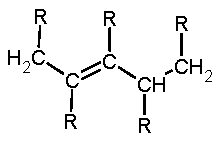
\includegraphics[width=80px]{pent3ene.pdf}
  \caption{Pent-3-ene}
  \label{fig:pent3ene}
\end{subfigure}%
\begin{subfigure}{.3\textwidth}
  \centering
  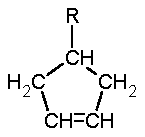
\includegraphics[width=60px]{RcycloPenteneHs.pdf}
  \caption{Cyclo-Pentene}
  \label{fig:cycloPen}
\end{subfigure}
\begin{subfigure}{.3\textwidth}
  \centering
  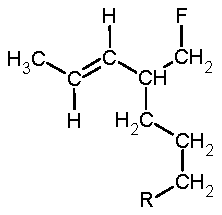
\includegraphics[width=80px]{pent3ene2propNOF.pdf}
  \caption{Pent-3-ene-2-propyl-1-F}
  \label{fig:propSub}
\end{subfigure}
\caption{The chemical structure of molecules in the datasets, R = H, F, OH or NH\textsubscript{2}}
\label{fig:Molecules}
\end{figure}
%GEOFF: Too much detail here?
We generated the following three data sets, with the first being used for training and the remaining used for testing. Each data set consists of a set of molecules, as defined by the bonding pattern between the atoms, and a set of distinct geometries of these molecules, as defined by distortions of the structure away from the equilibrium geometry. The geometric distortions are generated using a random uniform distribution of $\pm$0.5\AA\ for bond lengths and $\pm$10\textsuperscript{o} for bond angles.  This approach of uniform sampling generates highly distorted structures. To prevent inclusion of structures that are of little interest in chemical applications, structures are rejected if there are contacts closer than 3\AA\ between non-bonded atoms.  In addition, each molecular configuration is placed in 4 different electrical field environments (1 with no field + 3 different fields for X, Y and Z directions).
\begin{description}
%Matteus: I don't think the pent3ene test set ever gets shown in this paper, so we could perhaps delete it? We could delete it. The test set includes three distorted geometries for each molecule. 
\item[\textit{pent3ene}] 15 unique molecules corresponding to single substition of Pent-3-ene: we place a single substituent at one of the positions indicated by R in Figure~\ref{fig:pent3ene}, with all other R's being hydrogen (-H). The substituents are fluorine (-F), hydroxyl (-OH) and amine (-NH\textsubscript{2}). The training set includes, for each molecule, the equilibrium geometry and three distorted geometries. In addition, each geometry includes a random free rotation about the leftmost carbon-carbon single bond of Figure~\ref{fig:pent3ene}. 
\item[\textit{cycloPentene}]Includes cyclo-pentene and its three singly-substituted analogues (Figure~\ref{fig:cycloPen}), each in the equilibrium geometry and 4 distorted geometries. 
\item[\textit{pentPropylF}] Includes the three singly-substituted species of pent-3-ene-2-propyl-1-Fluorine (Figure~\ref{fig:propSub}), each in its equilibrium geometry and 7 distorted geometries. In addition, each geometry includes a random free rotation about the leftmost carbon-carbon single bond of Figure~\ref{fig:propSub}. 
\end{description}

%Geoff: Is R a form of regularization? 
% GJG: talk about how we train the policy: least squares, gradient descent, finite differences to deal with HF step
For each molecular instance, the steady-state density matrix, $\rho_n$, is obtained using a standard fixed-point algorithm~\citep{Pulay1980}. The learning objective is then defined as the sum of the distance of the density matrix, $\|\rho_i-\rho_n\|$, and the molecular energy, $|E(\rho_i)-E(\rho_n)|$ in Hartrees, from convergence. Because As in DIIS methods, it is likely desirable to have the coefficients of the linear combination of density matrices sum to one~\cite{scusceria} the following is added to the objective,
\begin{equation}
R^{(i)}_j =  w [(\sum \|\hat{c}^{(i)}_j\| - 1]
\end{equation}
where the weight $w$ was empirically adjusted to a value of 30.
The polcies are trained by using the trust-region reflective algorithm~\cite{Coleman1996} as implemented within Matlab.~\cite{Matlab} 


%GEOFF and MATTEUS: Is this single iteration DAgger? Original name was least-squares.. ok to change to no-induced-states? 
%MT: We could call it no-induced-states or naive approach
%GEOFF: This is likely to require in-person discussion. Why not just use the sequence from the DIIS algorithm, eliminating every nth instance to create an enhanced expert.
We use a heristic approach to generate a high-quality expert sequence. We first train a policy that takes the initial density matrix to the final density matrix $(\rho_0) \rightarrow \rho_n$, and use this to generate $\rho_1$. A policy is then trained on $(\rho_0, \rho_1) \rightarrow \rho_n$ and used to generate $\rho_2$, and so on. This approach is essentially single-iteration DAgger, targeting $\rho_n$, and will be referred to as the ``naive-supervised-learning'' policy. Every instance in the training data converges in less than 12 iterations, which is considerably faster than DIIS~\cite{Pulay1980} and so provides a high-quality expert demonstration. Enhanced expert demonstrations are created by eliminating the odd numbered iterations and DAgger is used to train a policy that mimics these enhanced demonstrations, as in Section~\ref{sec:policy}. To further expand the training data, expert demonstrations are constructed starting from two starting points, by setting $\rho_0$ of Algorithm~\ref{alg:hf} to 0 and to the identity matrix, ${\bf I}$. This leads to two different expert demonstrations for each molecular instance that sample substantially different states early in the trajectories. 

As a ``baseline'' policy for comparison, we use the simple policy in which the density matrix for iteration $i$ is the average of the density matrices from the past two iterations.

\section{RESULTS}


\begin{figure}[h!]
\centering
\begin{subfigure}{.5\textwidth}
  \centering
  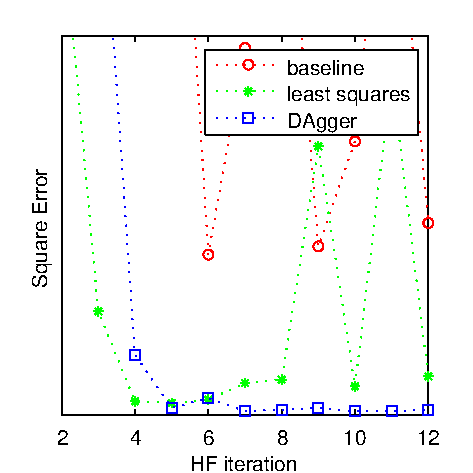
\includegraphics[scale=0.7]{cycloPen_pzero_test_12iter.pdf}
  \caption{$\rho_0 = 0$}
  \label{fig:cycloPen0}
\end{subfigure}%
\begin{subfigure}{.5\textwidth}
  \centering
  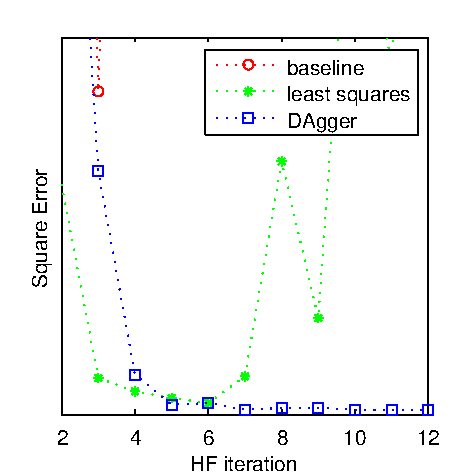
\includegraphics[scale=0.7]{cycloPen_peye_test_12iter.pdf}
  \caption{$\rho_0 = I$}
  \label{fig:cycloPenI}
\end{subfigure}
\caption{Error as a function of iteration tested on \textit{cycloPentene} dataset}
\label{fig:testcycloPen}
\end{figure}


Both the no-induced-states and DAgger policies converge in the first few iterations on the \textit{pent3ene} training dataset (data not shown). On the test data, both policies converge more rapidly and to lower final error than the baseline policy (Figure \ref{fig:testcycloPen} and \ref{fig:testpropSub}). However, DAgger leads to more robust behavior, including rapid convergence from both the  $\rho_0 = 0$ and $\rho_0 = I$ starting points. These results demonstrate that imitation learning can accelerate fixed-point iteration in a manner that generalizes to situations not included in the training data.

\begin{figure}[h!]
\centering
\begin{subfigure}{.5\textwidth}
  \centering
  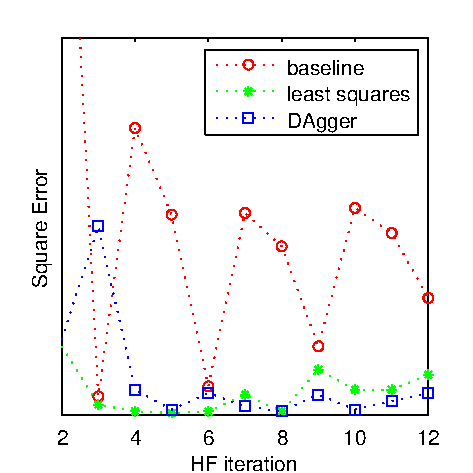
\includegraphics[scale=0.7]{propylsub_pzero_test_12iter.pdf}
  \caption{$\rho_0 = 0$}
  \label{fig:propSub0}
\end{subfigure}%
\begin{subfigure}{.5\textwidth}
  \centering
  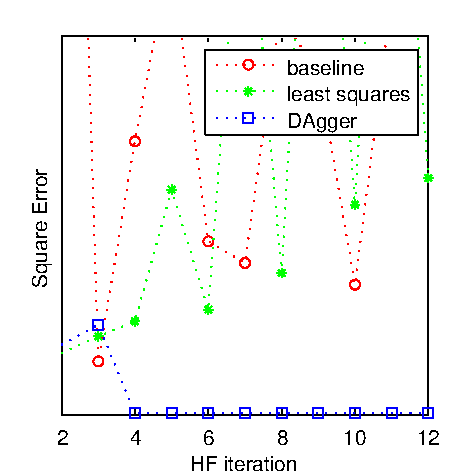
\includegraphics[scale=0.7]{propylsub_peye_test_12iter.pdf}
  \caption{$\rho_0 = I$}
  \label{fig:propSubI}
\end{subfigure}
\caption{Error as a function of iteration tested on \textit{pentPropylF} dataset}
\label{fig:testpropSub}
\end{figure}


\section{CONCLUSION}

The work explores a new application of imitation learning: accelerating the fixed-point iterations that are common in science and engineering. The mapping to imitation learning is quite general in that it requires only black-box access to the update function from an existing fixed-point algorithm.  The intuition is simple: we accelerate convergence by attempting to skip $\Delta-1$ out of every $\Delta$ calls to the original update function, replacing the skipped calls by a learned mapping.
The specific case considered here, the Hartree-Fock algorithm from quantum chemistry, allowed us to test the ability of policies trained on one situation (chemical system) to transfer to different situations (chemical systems). Our results  indicate successful transfer: imitation learning leads to policies that transfer better between systems than competing approaches.

\bibliography{refs}

\clearpage
\appendix
\section{The Hartree-Fock algorithm}
\label{app:hf}

% GJG: should put the formula for Fock matrix F(\rho) in enough detail to be implementable

The electron distribution is in principle given by the time-independent Schr\"{o}dinger equation, 
\begin{equation} \label{eq:schrodinger}
				\hat{H}\Psi = E\Psi
\end{equation}
Here $\Psi$ is the many-electron wave function, so that $\Psi^2(\mathbf r_1, \mathbf r_2, \ldots, \mathbf r_N)$ is the probability of finding the molecule's $N$ electrons at positions $\mathbf r_1, \mathbf r_2, \ldots, \mathbf r_N$. $\hat{H}$ is the Hamiltonian, a linear operator on the space of wave functions; $\hat H$ encodes the physical laws that govern the electrons.  Eq.~\ref{eq:schrodinger} is an eigenvalue problem: there are many solutions $\Psi$, each corresponding to a different energy level $E$.  We are interested in particular in the ground state, the solution of lowest energy.

Unfortunately, it is computationally prohibitive to solve the Schr\"odinger equation directly for all but the smallest molecules.  So, Hartree-Fock theory uses a mean-field approximation to replace the Schr\"odinger equation with the much simpler problem of finding the single-electron density $\rho(\mathbf r)$, then solves for $\rho(\mathbf r)$ by fixed-point iteration.  

In more detail, given a guess $\rho(\mathbf r)$ at the electron density, Hartree-Fock solves for \emph{molecular orbitals} $\phi_a(\mathbf r)$, each with associated energy $\epsilon_a$, by analyzing the behavior of a single electron under the mean field generated by $\rho(\mathbf r)$.  It then forms an updated electron density $\rho'$ by assuming that each of the molecule's $N$ electrons occupies one of these orbitals: no more than two electrons per orbital (one each with spin up and spin down, consistent with the Pauli exclusion principle), and occupying orbitals starting from the lowest energy ones (since we are interested in the ground state).

The molecular orbitals are solutions of a single-electron eigenvalue problem:
\begin{equation} \label{eq:fockSchrodinger}
				\hat{F}\phi_a({\bf r}) = \epsilon_a \phi_a({\bf r})
\end{equation}
Here $\hat F$ is the Fock operator, 
\begin{equation} \label{eq:fock}
\hat{F}(\rho) = \hat{h}_1 + \hat{G}(\rho({\bf r}))
\end{equation}
where $\hat{h}_1$ is the one-electron Hamiltonian, containing operators that account for the kinetic energy of the electrons and the interaction of the electrons with the nuclei, and $\hat{G}$ is an operator that captures the interaction between a single electron and the mean field based on the input density $\rho(\mathbf r)$.

%In Hartree-Fock theory, the distribution is described by the electron density $\rho({\bf r})$, which gives the probability of finding any electron at the position ${\bf r}$. Hartree-Fock theory derives from the time-independent Schr\"{o}dinger equation,
%\begin{equation} \label{eq:schrodinger}
%				\hat{H}\Psi = E\Psi
%\end{equation}
%where $\hat{H}$ is the Hamiltonian operator and the many-body, or many-electron, wave-function $\Psi$ is an eigenfunction of that operator. Different $\Psi$'s correspond to different quantum states of the system, but the goal of Hartree-Fock theory is to approximate the lowest-energy state. Hartree-Fock theory uses a mean-field approach to convert the many-body Schr\"{o}dinger equation to a one-electron problem,
%\begin{equation} \label{eq:fockSchrodinger}
%				\hat{F}\phi_a({\bf r}) = \epsilon_a %\phi_a({\bf r})
%\end{equation}
%where $\hat{F}$ is the Fock operator, $\phi_a({\bf r})$ are the molecular orbitals, which describe the possible quantum states of individual electrons, and $\epsilon_a$ are the molecular orbital energies. An approximation for the many-electron system is then constructed by assuming the $N$ electrons of the molecule occupy the lowest-energy orbitals, consistent with the Pauli exclusion principle restriction of placing at most two electrons (one with spin up and one with spin down) into any given molecular orbital. The Fock operator
%\begin{equation} \label{eq:fock}
%\hat{F}(\rho) = \hat{h}_1 + \hat{G}(\rho({\bf r}))
%\end{equation}
%where $\hat{h}_1$ is the one-electron Hamiltonian containing the operators that account for the kinetic energy of the electrons and the interaction of the electrons with the nuclei. $\hat{G}$ is an operator that captures the interaction between a single electron and the mean field resulting from all electrons. This mean field is constructed from the electron density, $\rho({\bf r})$. 

For computational purposes, the molecular orbitals, $\phi_a$ of Eq.~\ref{eq:fockSchrodinger} are written as a linear combination of basis functions,
\begin{equation}\label{eq:lcao}
\phi_a({\bf r}) = \sum_{i=1}^{N_{basis}} \chi_i({\bf r}) C_{i,a}
\end{equation}
%The set of basis functions, $\chi_i$, provides a finite-dimensional Hilbert space in which to obtain approximate solutions. In this space, 
The operators $\hat{F}$, $\hat{h}_1$, and $\hat{G}$, along with the density $\rho({\bf r})$, become symmetric matrices of dimension $N_{\rm basis}$, and Eq.~\ref{eq:fockSchrodinger} becomes a generalised matrix eigenvalue problem:
\begin{equation}\label{eq:fockMatrix}
F(\rho)c_a = Sc_a\epsilon_a
\end{equation}
where $F$ is the Fock matrix (with $F_{ij} = \langle \chi_i, \hat F\chi_j\rangle$) and $S$ is the matrix of inner products of the basis functions ($S_{ij} = \langle\chi_i,\chi_j\rangle$).  Assigning an electron to the orbital $\phi_a$ now corresponds to adding $c_a c_a^\top$ to the density matrix $\rho$.

% GJG: we're using both $c$ and $\phi$ to refer to molecular orbitals (differing in vector vs function form); but we use the same letter for $\hat F$ and $F$; seems inconsistent

%$\rho$ is the density matrix which expresses the electron density $\rho({\bf r})$ in the basis set and is given by $C^TC$. 

%Hartree-Fock scales nominally as $O(N_{\rm basis}^4)$ due to the evaluation of $\hat{G}$, although scalings closer to $N_{\rm basis}^3$ are routinely achieved by taking advantage of sparsity in construction of $\hat{G}$~\ref{?}.

% The corresponding fixed point iteration is shown in Algorithm~\ref{alg:hf}. Implementations differ with regards to the means used to construct the starting density matrix and, more importantly for the current study, with regards to the means used to construct a guess density matrix in the first line of the while loop. This is typically done by taking a linear combination of these past iterates. In the Direct Inversion in the Iterative Subspace (DIIS) method \citep{Pulay1980}, the linear coefficients are chosen by associating an error vector which each iterate and choosing coefficients that minimize the summed error. Various methods have been used to define the error vector and to find the linear combinations that minimize the predicted error~\citep{ADIIS,compScuseria,Alejandro2012}. However, how to generate linear combinations that lead to the fastest convergence remains an open question~\citep{Konstantin2002, Thorsten2011}. The current work retains the approach of using a linear combination of past iterates, but uses supervised learning to discover the optimal coefficients. 

\end{document}




